\documentclass[a4paper,12pt]{scrreprt}

\usepackage{scrhack}
\usepackage[utf8]{inputenc}
\usepackage[T1]{fontenc}
\usepackage{silence}
\WarningFilter{scrreprt}{Usage of package `fancyhdr'}
\usepackage{graphicx}
\usepackage{tikz}
\usepackage{times}
\usepackage{listings}
\usepackage{amssymb}
\usepackage{amsfonts}
\usepackage{amsmath}

% --------- 

\titlehead{Department of Informatics, University of Zürich}
\subject{\vspace*{2cm}MSc Thesis}
\title{Implementing Learned Indexes on 1 and 2 Dimensional Data}
\author{
  Neeraj Kumar, Nivedita Nivedita, Xiaozhe Yao\\[-5pt]
  \scriptsize Matrikelnummer: 19-759-570\\[-5pt]
  \scriptsize Email: \texttt{xiaozhe.yao@uzh.ch}
}
\date{\vspace*{2cm}January 11, 2010}
\publishers{
  \small supervised by \\ 
  Prof.\ Dr.\ Michael H. Böhlen and \\ Mr. Qing\ Chen \\[5cm]
  \begin{tikzpicture}[overlay]
    \node at (-3,-3) {
\includegraphics[height=1.5cm]{IFIlogo}};
    \node at (7,-3) {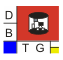
\includegraphics[height=1.5cm]{dbtgBW}};
  \end{tikzpicture}
}

% --------- 

\newtheorem{definition}{Definition}
\newtheorem{example}{Example}
\newtheorem{theorem}{Theorem}
\newtheorem{lemma}{Lemma}


% --------- 

\begin{document}

\maketitle

\begin{abstract}
	
\end{abstract}

\chapter*{Abstract}

\chapter{Introduction}

Over the years, indexes have been widely used in databases to improve the speed of data retrieval. In the past decades, the database indexes generally fall into hand-engineered data structures and algorithms, such as B-Tree, KD-Tree, Hash Table, etc. These indexes have played an important role in databases and have been widely used in modern data management systems (DBMS). Despite their success, they do not consider the distribution of the database entries, which might be helpful in designing faster indexes.

For example, if the dataset contains integers from $1$ to $1$ million, the key can be used directly as an offset. With the key used as an offset, the values with the key can be retrieved in $\mathcal{O}(1)$ time complexity. Compared with B-Tree, which always takes $\mathcal{O}(\log n)$ time complexity for the same query. At the same time, by using the key as an offset directly, we do not need any extra overhead regarding memory space, where the B-Tree needs extra $\mathcal{O}(n)$ space complexity to save the tree.

From the above example, we found there are two promising advantages of learned indexes over hand-engineered indexes:
\begin{enumerate}
  \item Learned indexes may be faster when performing queries, especially when the number of entries in the database are extremely huge.
  \item Learned indexes may take less memory space, as we only need to save the model with constant size.
  \end{enumerate}
  
 We will explore and analyse these two advantages qualitatively in the \textit{chapter 5}. 

Nowadays, to leverage these two advantages, researchers proposed learned indexes \cite{kraska2018case}, where machine learning techniques are applied to automatically learn the distribution of the database entries and build the data-driven indexes. This approach has been shown to be powerful and competitive compared with hand-engineered indexes, such as B-Tree.

In this report, we explore the development of database indexes, from hand-engineered indexes to the learned index. After that, we explore the possibilities of using complex convolutional neural networks as database indexes. This report is organised into the following chapters:

\begin{enumerate}
	\item \textbf{Introduction}. In this chapter, we illustrate the organisation of this report. Besides, we go through the modern computer systems and introduce the general information about database indexes. 
	\item \textbf{Traditional Indexes used in Database}. In this chapter, we analyse one of the most important traditional index: B-Tree. We go through its motivation, algorithms, advantages and disadvantages. Besides, we explore some other traditional indexes such as B+ Tree briefly.
	\item \textbf{Baseline Learned Indexes}. In this chapter, we build our first learned index with fully connected neural networks. We demonstrate how it works, explore its properties and analyse its advantages and disadvantages. 
	\item \textbf{Recursive Model Index}. Proposed by T.Kraska \cite{kraska2018case},  Recursive Model Index (RMI) is one of the most popular model used as learned index. In this chapter, we will explain its mechanism, demonstrate its algorithm and qualitatively analyse its pros and cons. 
	\item \textbf{2D Learned Index}. Until so far, we only work with $1$-dimensional data. 2-D indexes is also important in many applications. For example, in a location query, where users want to find out all the stores in a certain rectangle, all stores are indexed by 2-D keys, i.e. the coordinates. In this chapter, we will explore how 2-D keys are indexed and arranged using a learned fashion.
	\item \textbf{Learned Indexes with Convolutional Neural Network}. In this chapter, we discover the possibilities of using convolutional neural network (CNN) as database index. 
\end{enumerate}

\section{Terminologies}

In the following chapters, we will use the following terminologies

\textbf{Index model} is a function that maps the index of a row of data into the location (e.g. page index) of the data. For example, in one-dimensional case, the index models include B-Tree, Linear Regression models, etc.

\textbf{Key} is a special attribute in the database that could identify a record. In our work, the key could be a scalar in one-dimensional case, or a $(x,y)$ pair in two-dimensional case.

\textbf{Order of a tree} is the maximum number of children that a node can have.

\textbf{Internal node} is any node of a tree that has child nodes and is not a root node.

\textbf{Leaf node} is any node that does not have child nodes.

\textbf{Level} of a node is defined as the number of edges between this node and the root node.


\section{Motivation}

In traditional database indexes, the complexity for locating an item is usually bounded by some function related to the total number of elements. For example, with a B-Tree, an item can be found within $\mathcal{O}(\log n)$ time complexity. In the meantime, saving a B-Tree as index takes $n$ space complexity. With the rapid growing of the volume of data, $n$ becomes much larger than ever before. Hence, the big data era is calling for a database index that have constant complexity in both time and space.

To achieve such a goal, the distribution of the data is important. For example, assume that the data is fixed-length records over a set of continuous integers from 1 to 100 million, the conventional B-Tree index can be replaced by the keys themselves, making the query time complexity an $\mathcal{O}(1)$ rather than $\mathcal{O}(\log n)$. Similarly, the space complexity would be reduced from $\mathcal{O}(n)$ to $\mathcal{O}(1)$. This example shows that with the knowledge of the distribution of the data, it is possible to locate the item in database in constant time.

Formally, we define the index of each record as $x$ and the corresponding location as $y$ and we represent the whole data as $(X, Y)$ pairs with the total number of pairs defined as $N$. We could then normalise the $Y$ into $\tilde{Y}\in[0,1]$ so that the $\tilde{y}$ represents the portion of the $y$ among the whole $Y$. With these definitions, we can then define a function $F:X\to \tilde{Y}$ that maps the index into the portion of the $y$. We have $y=F(x)* N$. As the output of this function can be considered as the probability of $X\leq x$, we can regard this function $F(x)$ as the cumulative distribution function (CDF) of $X$, i.e. $F(x)=\mathbb{P}(X\leq x)$. Now that $N$ is determined by the length of data records, we only need to learn such CDF and we called the learned CDF function as \textbf{learned index model}.

From the perspective of the distribution of data records, our previous example can be rephrased as following. Our data records are $(X, Y)$ pairs with a linear relation, i.e. $y=x, \forall y\in Y$. We are looking for a function $F$ such that $y=x=F(x)* N$, and hence we end up with $F(x)=\frac{1}{N}*x$. If we use this linear function $F(x)$ as the index model, then we could locate the data within $\mathcal{O}(1)$ time complexity and we only need to store the total number of records as the only parameter. Compared with B-Tree and other indexes, the advantages are enormous.

Even though there might be potential advantages, the learned index model has several assumptions, as listed below.
\begin{enumerate}
	\item All data records are stored in memory. 
	\item All data records are sorted by $X$.
	\item All data records are stored statically in database, hence we do not take insertion and deletion into consideration.
\end{enumerate}




\chapter{Traditional Indexes used in Database}

\section{B-Tree}
B-Tree and its variants have been widely used as indexes in
databases. For example, the PostgreSQL uses B-Tree as its index. B-Trees
can be considered as a natural generalisation of binary search tree. In
binary search tree, there is only one key and two children possible in
it's internal node. However, an internal node of B-Tree can contain
several keys and children. The keys in a node serve as dividing points
and separate the range of keys. With this structure, we make an
multi-way decision based on comparisons with the keys stored at the node
\(x\). The image below illustrates a simple B-Tree.

In this section, we will introduce the construction and query processes
of B-Trees and then analyse their properties.

\subsection{Motivation}

In computers, the memories are organised in an hierarchical way. For example, a classical computer system consists three layers of memory: the CPU cache, main memory and the hard disk. In such a system, the CPU cache is the fastest but the most expensive while and hard disk is the cheapest but also the slowest. When querying for an item, the CPU will first try to fetch it from the CPU cache. If not there the CPU will then try to fetch it from the main memory, and then the hard disk.

%TODO: Some statements are needed to show the data is stored in blocks in the memory.

At the same time, the traditional hard disk drive (HDD) is made by a moving mechanical parts.

%TODO: Illustrate the mechanical structure.

%TODO: I don't think we need this part anymore? Removing the motivation might be helpful...

In summary, there are two properties in classical computer systems that we need to take into account:

\begin{enumerate}
	\item The memory is not flat, meaning that memory references are not equally expensive. 
	\item 
\end{enumerate}

\subsection{Definition and Terms}

Before we formally define B-Trees, we assume the following terms:

\begin{itemize}
\item
  \textbf{Keys}: The key in database is a special attribute that could
  identify a row in the database. In our work, each key corresponds to a
  \textbf{value} and forms a key-value pair.
\item
  \textbf{Internal Node}: An internal node is any node of the tree that
  has child nodes.
\item
  \textbf{Leaf Node}: A leaf node is any node that does not have child
  nodes.
\end{itemize}

Each node in a B-Tree has the following attributes:

\begin{itemize}
\item
  \(x.n\) is the number of keys currently stored in the node \(x\).
\item
  Inside each node, the keys are sorted in nondecreasing order, so that
  we have \(x.keys_1\leq x.keys_2\leq\cdots\leq x.keys_{x.n}\).
\item
  \(x.leaf\), a Boolean value determines if current node is a leaf node.
\end{itemize}

With these properties, A B-Tree \(T\) whose root is \(T.root\) have the
following properties:

\begin{itemize}
\item
  Each internal node \(x\) contains \(x.n+1\) children. We assume the
  children are \(x.c_1,\cdots,x.c_{x.n+1}\).
\item
  The nodes in the tree have lower and upper bounds on the number of
  keys that can contain. These bounds can be expressed in terms of a
  fixed integer \(t\)
\end{itemize}

\subsection{Insertion of B-Tree}

When inserting keys into a binary search tree, we search for the leaf
position at which to insert the new key. However, with B-Tree, we cannot
simply find the position, create a new node and insert the value because
the tree will be imbalanced again. Hence, in this section we illustrate
an operation that splits a full node around its median key



\chapter{Baseline Learned Indexes}

\section{Baseline Models}

Our baseline model is a two layer fully connected neural network. Before
constructing the neural network, we will try to theoretically analyze
the requirements in such a neural network serving as database index.


\subsection{Neural Network Settings}

The input (key) to our neural network is a scalar, and the expected
output of the neural network is the position of the given input. We
assume the following parameters in the neural network:

\begin{itemize}
\item
  The weight in the \(i\)th layer \(w^{(i)}\).
\item
  The bias in the \(i\)th layer \(b^{(i)}\).
\item
  The activation function after the \(i\)th layer \(z^{(i)}\).
\end{itemize}

For example the output of the first layer will be
\(z^{(1)}(w^{(1)}x+b^{(1)})\).


\subsection{Activation Functions}

\begin{itemize}
\item
  If we use identity activation function, i.e.~\(z^{(i)}(x)=x\), then no
  matter how many layers are there, the fully connected neural network
  falls back to a linear regression.

  \textbf{Proof:} The output of the first layer, with identity
  activation function, will be
  \(z^{(1)}(w^{(1)}x+b^{(1)})=w^{(1)}x+b^{(1)}\). Then the output will
  be the input of the next layer, and hence the output of the second
  layer will be
  \(z^{(2)}(w^{(2)}(w^{(1)}x+b^{(1)})+b^{(2)})=w^{(2)}w^{(1)}x+w^{(2)}b^{(1)}+b^{(2)}\).
  Similar induction can be obtained for multiple layers. Hence if we use
  identity activation, the trained neural network will fall back to a
  linear regression. The visualization below shows our lemma is correct.
\item
  With ReLU (Rectified Linear Unit) as activation function
  i.e.~\(z^{(i)}(x)=\text{max}(0,x)\), then the fully connected neural
  network falls back to a piecewise linear function.

  \textbf{Proof:} The output with ReLU activation function, will be
  \(z^{(1)}(w^{(1)}x+b^{(1)})=\text{max}(w^{(1)}x+b^{(1)}, 0)\). Then
  the output will be the input of the next layer, and hence the output
  of the second layer will be
  \(z^{(2)}(w^{(2)}(w^{(1)}x+b^{(1)})+b^{(2)})=\text{max}(w^{(2)}w^{(1)}x+w^{(2)}b^{(1)}+b^{(2)},0)\).
  Similar induction can be obtained for multiple layers. Hence if we use
  identity activation, the trained neural network will fall back to a
  piecewise linear function. The visualization below shows our lemma is
  correct.
\end{itemize}

\subsection{Monotonicity}

\chapter{Recursive Model Index (RMI)}

\section{Introduction}

%TODO: there should be some graph to demonstrate the last-mile problem.

In our baseline models, it is not very difficult to reduce the mean square error from millions to thousands. However, it is much harder to reduce it from thousands to tens. This is the so called last-mile problem.

In order to solve this problem, recursive model index was proposed \cite{kraska2018case}. The idea is to split the whole set of data into smaller pieces and assign each piece an index model.

\section{Definitions}


Similar to a tree, we define the following terms in a recursive model:

\begin{enumerate}
	\item \textbf{Node Model}. Every node is responsible for making decisions with given input data. In one dimensional case, it can be regarded as a function $f:\mathbb{R}\to\mathbb{R}, x\to y$ where $x$ is the input index and $y$ is the corresponding page block. In principle, each node can be implemented as any machine learning model, from linear regression to neural network, or a traditional tree-based model, such as B-Tree.
	\item \textbf{Internal Node Model}. Internal nodes are all nodes except for leaf nodes and the root node. Every internal node receives a certain part of training data from the full dataset, and train a model on it. 
\end{enumerate}

In the following sections, we will use the notations defined below:
\begin{enumerate}
	\item $N_M^{(i)}$ is the number of models in the $i$th stage.
	%TODO: more notations
	%TODO: modify algorithms accordingly
\end{enumerate}

\section{Training}

In order to construct a recursive model, we need to have several parameters listed below:
\begin{enumerate}
	\item The training dataset, notated as $(X, Y)$ with entries notated as $(x,y)$.
	\item The number of stages, notated as $N_S$. It is an integer variable.
	\item The number of models at each stage, notated as $N_M$. It is a list of integer variable. $N_M^{(i+1)}$ represents the number of models in the $i$th stage.
	\item 
\end{enumerate}

The training process of recursive model is a up-bottom process. There will be only one root model that receives the whole training data. After the root model is trained, we iterate over all the training data and predict the page by the root model. After the iteration, we get a new set of pairs $(X, Y_0)$. Then we map $\forall y_0\in Y_0$ into the selected model id in next stage by $\texttt{next}=y_0 * N_M^{(i+1)}/\texttt{max(Y)}$.

\begin{algorithm}[H]
    \SetAlgoLined
    \SetKwInOut{Input}{input}
    \Input{\texttt{num\_of\_stages; num\_of\_models; types\_of\_models; x; y}}
     \texttt{trainset=[[(x,y)]]} \\
     \texttt{stage$\gets 0$} \\
     \While{\texttt{stage} \textless \texttt{num\_of\_stages}}{
      \While{\texttt{model} \textless \texttt{num\_of\_models[stage]}} {
        \texttt{model.train(trainset[stage][model])} \\
        \texttt{models[stage].append(model)}
      }
      \uIf{not last stage} {
        \For{$i\gets0$ \KwTo $len(x)$}{
            	\texttt{model=models[output from previous stage]} \\
            	\texttt{output=model.predict(x[i])} \\
            	\texttt{next=output * num\_of\_models[stage+1]/max\_y} \\
            	\texttt{trainset[stage+1][next].add((x[i],y[i]))}
        }
      }
     }
     \caption{Training of Recursive Model Index}
\end{algorithm}

\section{Prediction}

\begin{algorithm}[H]
    \SetAlgoLined
    \SetKwInOut{Input}{input}
    \Input{\texttt{x; models; num\_of\_stages; max\_y}}
     \texttt{stage$\gets 0$} \\
 	 \texttt{next\_model$\gets 0$} \\
     \While{\texttt{stage} \textless \texttt{num\_of\_stages}}{
        \texttt{output = model.predict(x)} \\
        \texttt{next\_model=output*len(models[stage+1])/max\_y}\\ 
      \uIf{last stage} {
		\texttt{y = next}
      }
     }
     \caption{Training of Recursive Model Index}
\end{algorithm}



\bibliographystyle{alpha}
\bibliography{refs}

\end{document}
